\documentclass[12pt]{article}
\usepackage{cite}
\usepackage{mathtools} %% includes amsmath
\usepackage{amssymb,amsfonts}
\usepackage{algorithmic}
\usepackage{textcomp}
\usepackage{xcolor}
\usepackage{physics}
\usepackage{graphicx,graphics}
\setlength{\oddsidemargin}{0.25in}
\setlength{\evensidemargin}{-0.25in}
\setlength{\topmargin}{-.5in}
\setlength{\textheight}{9in}
\setlength{\parskip}{.1in}
\setlength{\parindent}{2em}
\setlength{\textwidth}{6.25in}

\newcommand{\N}{\mathcal{N}}
\newcommand{\rv}{\vb{r}}
\newcommand{\rhat}{\hat{\rv}}

\title{Notes on b-spline implementation}
\date{\today}
\author{Robert J. Harrison}
 
\begin{document}

\maketitle

This document is initially looking at the b-spline-only implementation. 

The functional form is
\begin{eqnarray}
  f(\vb{r}) & = & \sum_{l m} \N_{lm}(\rhat) r^l R_{lm}(r) \\
  R_{lm}(r) & = & \sum_i c_{lmi} b_i(r)
\end{eqnarray}
Comments:
\begin{itemize}
\item The usual spherical coordinate system with $r = |\rv| \in [0,\infty]$, $\theta \in [0,\pi]$ with $z=r \cos \theta$, and $\phi \in [0,2 \pi]$.
\item The $\N_{lm}(\rhat)$ where $\hat{r}$ is the unit vector are the real solid spherical harmonics of Yang normalized so that
\begin{eqnarray}
  \int_0^{2 \pi} d\phi \int_0^\pi d\theta \sin \theta  \N_{lm} (\hat{r}) \N_{l^\prime m^\prime}(\hat{r})  & = & \delta_{l l^\prime} \delta_{m m^\prime}
\end{eqnarray}
Note that Yang does not normalize his harmonics for ease of computing various quantities.  However, we need radial and angular components to be normalized so we can perform numerical thresholding without having to keep track of normalization constants, which for Yang's harmonics (denoted $N_{lm}$)  can be truly huge ($O(10^{2l})$ or worse).  Yang's normalization also results in $N_{10}=z$ but $N_{11}=-x/2$ and $N_{1-1}=-y/2$ and so potentially breaks symmetry.  
\item $b_i(r)$ is a b-spline basis function defined on knots that include the origin. 
\item We separate out the factor $r^l$, with these consequences:
  \begin{enumerate}
  \item Ensures correct behavior near the origin.  If we bundled $r^l$ into $R(r)$ then then degree of the b-spline basis would have to be greater than or equal to the maximum angular momentum for an exact representation.  Since some of the algorithms scale highly non-linearly with the order, we want to use order circa 8-12.
  \item Since $r^l \N_{lm}(\rhat) = n_{lm} N_{lm}(\rv) \propto  x^i y^j z^k$ for $i+j+k=l$), we expect $R_{lm}(r)$ to tend to a non-zero constant near the origin (except for the Dirac $s$ components that are weakly singular there).  
  \item Facilitates convolution with the Coulomb and Helmholtz GFs so we can exactly cancel factors such as $r^{-l}$.
  \item Derivatives are also easier.
  \end{enumerate}
\end{itemize}

{\bf todo:} Revisit the decision to normalize the harmonics.  Maybe it is an unnecessary complication.

\section{B-splines}

Refer to standard references for details of the basis and associated algorithms.  The basis is specified by 
\begin{itemize}
\item $p$ --- the degree of the basis, and
\item a vector of unique knots.
\end{itemize}
We employ the full set of b-splines over a vector of unique knots.  The definition of the full basis requires a vector with the knots padded on either end by the last knot repeated $p$ times.  Note we actually store this vector ($t$ in the code) since it makes algorithms to compute with b-splines much easier. 

Thus, for a basis of degree $p$ (order $p+1$) and $m$ unique knots 
\begin{itemize}
\item they form (in the limit of dense knots or infinite order) a complete basis over the interval with approximation error $O\left(h^{r+p+1}\right)$ for a function with $r$ continuous derivatives 
\item the basis has $C_{p-1}$ continuity, meaning its value and all derivatives up to $p-1$ are continuous
\item the number of padded knots is $m + 2p$
\item the total number of basis functions is $m + p - 1$ 
\item the number of basis functions non-zero over a given knot interval is $p + 1$
\item each spline is non-zero over $p+1$ knot intervals and is controlled by $p+2$ knot values
\item each spline is positive within its support (and zero outside)
\item the sum of all splines at each knot is unity by construction
\item the fully interior sides of splines are zero at the end of their support along with their derivatives up to $p-1$
\item splines touching the edge have lower number of vanishing derivatives, and only the first/last splines have non-zero values at the end points (and these values will be one by construction).
\end{itemize}

\subsection{Radial knots}

We are computing on the interval $[0,L]$ which we can obtain by scaling the unit interval $[0,1]$ by $L$.  By defining monotonically-increasing maps from $[0,1]$ back onto $[0,1]$ we can nest transformations.    For $n$ knots
\begin{itemize}
\item Uniform knots $x(i) = i/(n-1)$
\item Chebyshev-like knots (that include the end points and concentrate quadratically on both ends) $x(i) = (1-\cos \pi i / (n-1))/2$
\item Half Chebyshev-like knots (that only concentrate on the left) $x(i) = 1 - \cos \pi i / (2(n-1))$
\item Rational function similar to half-Cheby $x(i) = i^2 (1+a) / (1 + ai)$
\item Geometric
\item Power
\end{itemize}

The below figures display the basis with 15 knots, order 6, with uniform and rational knots.

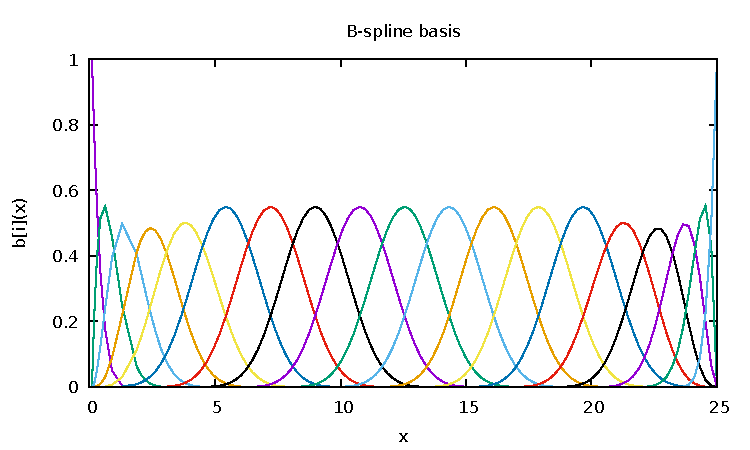
\includegraphics[width=.9\linewidth]{basis.pdf}

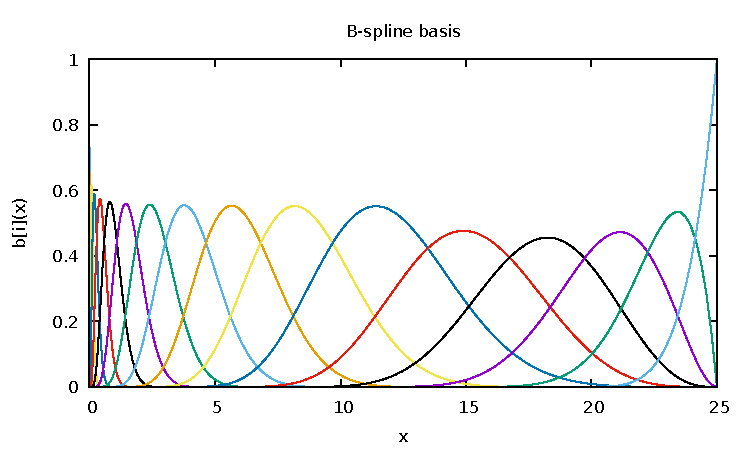
\includegraphics[width=.9\linewidth]{basis-non-uni.pdf}

\section{Radial derivatives}

The 

\section{Angular quadrature}
In double precision, the Lebedev or Beylkin rules suffice.  For higher precision, to exactly integrate angular momenta up to $L$  we employ
\begin{itemize}
\item $\theta$: The Gauss-Legendre rule of order $k_\theta = L/2 + 1$ scaled to $[0,\pi]$ ($k$ points can exactly integrate up to $x^{2k-1}$)
\item $\phi$: $k_\phi = \max(1,2 L)$ equispaced points in $[0,2 \pi)$ ($\phi_i = 2 i \pi / k_\phi$) with weights $2 \pi / k_\phi$.
 \item The total number of points $k_\theta k_\phi = (l_{\mbox{max}} + 1) \max(4 l_{\mbox{max}},1) $.
\end{itemize}
We choose $L = \max(1, 2 l_{\mbox{max}})$, where $l_{\mbox{max}}$ is the maximum angular momentum in the basis, so that we can exactly integrate products.  Table \ref{tab:GLnpts} illustrates how the required number of points scales with $l$ for each quadrature rule.

{\bf todo:} Add Beylkin's rule 

\begin{table}
  \begin{center}
  \caption{Number of angular quadrature points employed for select angular momenta} \label{tab:GLnpts}
  \begin{tabular}{ccc}
    $l_{\mbox{max}}$ & Lebedev & GL  \\ \hline
    0 & 6 & 1 \\
    1 & 6 & 8 \\
    2 & 14 & 24 \\
    3 & 26 & 48 \\
    4 & 38 & 80 \\
    5 & 50 & 120 \\
    6 & 74 & 168 \\ \hline
  \end{tabular}
  \end{center}
\end{table}

\section{Radial quadrature in the b-spline basis}

Between knots, each basis function is just a polynomial of degree $p$.  Since Gauss-Legendre (GL) quadrature with $n$ points can exactly integrate polynomials up to degree $2n-1$, these are the required number of points for various scenarios
\begin{itemize}
\item $\int r^l b_i(r) dr$ --- $n \ge (l+p-1)/2$
\item $\int r^l b_i(r) b_j(r) dr$ --- $n \ge (l+2p-1)/2$
\end{itemize}
Pre-tabulated are quadrature points and weights with $n=p+2$, which is adequate for integrals of up to the form $\int r^3 b_i(r) b_j(r)$ which is enough to construct all of the matrices needed to solve atoms.

\section{Projection}

Projecting $f(\vb{r})$ into the representation is accomplished by first integrating over the angular variables with

\begin{eqnarray}
  \int_0^{2 \pi} d\phi \int_0^\pi d\theta \sin \theta  \N_{lm} (\hat{r}) f(\vb{r}) & = & R_{lm}(r) 
\end{eqnarray}
With quadrature points on the unit sphere $\rhat_\mu$ with
weights $\omega_\mu$ and radial points $r_\nu$ , this becomes
\begin{eqnarray}
  R_{lm}(r_\nu) & = & \sum_\mu \omega_\mu \N_{lm} (\rhat_\mu) f(r_\nu \rhat_\mu)
\end{eqnarray}

The inversion from the function sampled at the grid points can be performed in several ways, paying attention to the ill-conditioning near the origin for the non-zero angular momenta.

By limiting the first (or last) $n$ basis functions the first $n$ derivatives can be forced to be zero on the left (or right).  
\begin{itemize}
\item $n=0$ no boundary conditions,
\item $n=1$ function value is forced to zero,
\item $n=2$ function value and first derivative are forced to zero,
\item etc.
\end{itemize}

\subsection{Weighted least squares and normal equations}
Adds a penalty to make the problem overall better conditioned and uses the normal equations.  For each $(l,m)$ the LSQ problem is to minimize
\begin{eqnarray}
  \sum_\nu  w(r_\nu) \left( R(r_\nu) - \sum_i c_i b_i(r_\nu) \right)^2 + \lambda \sum_i c_i^2
\end{eqnarray}
in which the weight is presumably to be chosen as $w(r)=r^2$.

The penalty term has little effect if $\lambda < \epsilon^2 / \sum_i c_i^2$. 

Setting the variation wrt $c_i$ to zero yields
\begin{eqnarray}
  0 & = & - 2 \sum_\nu  w(r_\nu) b_i(r_\nu) \left( R(r_\nu) - \sum_j c_j b_j(r_\nu) \right) + 2\lambda c_i
\end{eqnarray}
Tidying up yields
\begin{eqnarray}
  \sum_j \left( \sum_\nu w(r_\nu) b_i(r_\nu) b_j(r_\nu) \right) c_j + \lambda c_i & = & \sum_\nu  w(r_\nu) b_i(r_\nu)  R(r_\nu) \\
  \left( A + \lambda I \right) c & = & b ~ ~\mbox{with} \\
  a_{ij} & = & \sum_\nu w(r_\nu) b_i(r_\nu) b_j(r_\nu) \\
  b_i & = & \sum_\nu  w(r_\nu)  b_i(r_\nu) R(r_\nu) 
\end{eqnarray}

\subsection{Weighted least squares without using normal equations}

We can use a least-squares solver to determine $c$ in
\begin{eqnarray}
  w(r_\nu) \sum_i b_i(r_\nu) c_i \approx w(r_\nu) R(r_\nu).
\end{eqnarray}
However, it is much more convenient to construct using SVD the pseudo-inverse ($M$) of the matrix
\begin{eqnarray}
 a_{\nu i} & = & b_i(r_\nu) w(r_\nu) 
\end{eqnarray}
The b-spline basis is strongly linearly independent so there so there should always be a clear divide between zero and non-zero singular values and you can just use the expected number of non-zero singular values.

The fit is obtained directly with a matrix-vector product of $M$ acting on the vector of weighted function values evaluated at the (over-sampled) radial points.

\subsection{Projection into the b-spline basis}

Starting from 
\begin{eqnarray}
  \sum_j b_j(r) c_j \approx R(r)
\end{eqnarray}
we project from the left by $b_i(r)$ to obtain
\begin{eqnarray}
  \sum_j \left\langle b_i \middle| b_j\right\rangle c_j & \approx & \left\langle b_i \middle| R \right\rangle
\end{eqnarray}
The matrix on the left is just the overlap matrix ($S$) and we expand the integrals on the right using GL quadrature
\begin{eqnarray}
\left\langle b_i \middle| R \right\rangle = \sum_\nu b_i(r_\nu) \omega_\nu  R(r_\nu)
\end{eqnarray}
Hence, the fitting matrix ($M$) is given by
\begin{eqnarray}
   M & = & S^{-1} B
\end{eqnarray}
with
\begin{eqnarray}
  b_{i \nu} & = & b_i(r_\nu) \omega_\nu 
\end{eqnarray}

\section{Convolution with an integral operator}

Angular part is diagonal, so focus here on the radial part.

\section{Solid harmonics}

The functions $\N_{lm}(\vb{r})$ are normalized versions of the solid harmonics of Yang ($N_{lm}$).  The unnormalized versions are defined by the recursions (with $m\ge 0$) (the first two are used to recur up the diagonal $m=\pm l$ and the next two are then used to recur $l$ down from $l=m$ to $l=0$ (I inserted commas in the subscripts for clarity)
\begin{eqnarray}
  N_{0,0} & = & 1 \\
  N_{l, l} & = & -\frac{1}{2 l} \left(x N_{l-1,l-1} - y N_{l - 1, -(l - 1)}\right) \\
  N_{1,-l} & = & -\frac{1}{2 l} \left(y N_{l-1,l-1} + x N_{l - 1, -(l - 1)}\right) \\ 
  N_{l, m} & = & \frac{1}{(l+m) (l-m)} \left((2 l-1) z N_{l-1, m}-r^2  N_{l-2, m} \right) \\
  N_{l, -m}& = & \frac{1}{(l+m) (l-m)} \left((2 l-1) z N_{l-1, -m}-r^2 N_{l-2, -m} \right) 
\end{eqnarray}
with normalization constants
\begin{eqnarray}
  n_{lm} & = & \frac{\sqrt{(2 l +1) \left(l +{| m |}\right)! \left(l -{| m |}\right)!}  2^{-(1 + \delta_{0 m})/2}}{\sqrt{\pi}} .
\end{eqnarray}
The normalized harmonics are then
\begin{eqnarray}
  \N_{lm}(\vb{r}) & = & n_{lm} N_{lm}(\vb{r}).
\end{eqnarray}
The normalization is in the sense that an integral over the unit sphere yields
\begin{eqnarray}
  \int_0^{2 \pi} d\phi \int_0^\pi d\theta \sin \theta  \N_{lm} (\hat{r}) \N_{l^\prime m^\prime}(\hat{r})  & = & \delta_{l l^\prime} \delta_{m m^\prime} .
\end{eqnarray}
We tabulate the normalization constants and their reciprocals, so we can internally use the simple formulae of the unnormalized harmonics.

Note that $\N_{lm}(\vb{r}) = r^l N_{lm}(\rhat)$.

The first few unnormalized solid harmonics are
\begin{eqnarray}
N_{0, 0} & = &  1  \nonumber \\
N_{1, -1} & = &  -\frac{y}{2}  \nonumber \\
N_{1, 0} & = &  z  \nonumber \\
N_{1, 1} & = &  -\frac{x}{2}  \nonumber \\
N_{2, -2} & = &  \frac{y x}{4}  \nonumber \\
N_{2, -1} & = &  -\frac{z y}{2}  \nonumber \\
N_{2, 0} & = &  -\frac{r^{2}}{4}+\frac{3 z^{2}}{4}  \nonumber \\
N_{2, 1} & = &  -\frac{z x}{2}  \nonumber \\
N_{2, 2} & = &  \frac{x^{2}}{8}-\frac{y^{2}}{8}  \nonumber \\
N_{3, -3} & = &  -\frac{1}{16} x^{2} y +\frac{1}{48} y^{3}  \nonumber \\
N_{3, -2} & = &  \frac{z y x}{4}  \nonumber \\
N_{3, -1} & = &  \frac{y \left(r^{2}-5 z^{2}\right)}{16}  \nonumber \\
N_{3, 0} & = &  -\frac{1}{4} r^{2} z +\frac{5}{12} z^{3}  \nonumber \\
N_{3, 1} & = &  \frac{x \left(r^{2}-5 z^{2}\right)}{16}  \nonumber \\
N_{3, 2} & = &  \frac{1}{8} z \,x^{2}-\frac{1}{8} z \,y^{2}  \nonumber \\
N_{3, 3} & = &  -\frac{1}{48} x^{3}+\frac{1}{16} y^{2} x  \nonumber
\end{eqnarray}

The first few normalized solid harmonics are
\begin{eqnarray}
\N_{0, 0} & = &  \frac{1}{2 \sqrt{\pi}}  \nonumber \\
\N_{1, -1} & = &  -\frac{\sqrt{3} y}{2 \sqrt{\pi}} \nonumber \\
\N_{1, 0} & = &  \frac{\sqrt{3} z}{2 \sqrt{\pi}} \nonumber \\
\N_{1, 1} & = &  -\frac{\sqrt{3} x}{2 \sqrt{\pi}} \nonumber \\
\N_{2, -2} & = &  \frac{\sqrt{15} y x}{2 \sqrt{\pi}} \nonumber \\
\N_{2, -1} & = &  -\frac{\sqrt{15} z y}{2 \sqrt{\pi}} \nonumber \\
\N_{2, 0} & = &  -\frac{\sqrt{5} \left(r^{2}-3 z^{2}\right)}{4 \sqrt{\pi}} \nonumber \\
\N_{2, 1} & = &  -\frac{\sqrt{15} z x}{2 \sqrt{\pi}} \nonumber \\
\N_{2, 2} & = &  \frac{\sqrt{15} \left(x^{2}-y^{2}\right)}{4 \sqrt{\pi}} \nonumber \\
\N_{3, -3} & = &  -\frac{3 \sqrt{70} y \left(x^{2}-\frac{y^{2}}{3}\right)}{8 \sqrt{\pi}} \nonumber \\
\N_{3, -2} & = &  \frac{\sqrt{105} z y x}{2 \sqrt{\pi}} \nonumber \\
\N_{3, -1} & = &  \frac{y \left(r^{2}-5 z^{2}\right) \sqrt{42}}{8 \sqrt{\pi}} \nonumber \\
\N_{3, 0} & = &  -\frac{3 \sqrt{7} z \left(r^{2}-\frac{5 z^{2}}{3}\right)}{4 \sqrt{\pi}}  \nonumber \\
\N_{3, 1} & = &  \frac{x \left(r^{2}-5 z^{2}\right) \sqrt{42}}{8 \sqrt{\pi}} \nonumber \\
\N_{3, 2} & = &  \frac{\sqrt{105} z \left(x^{2}-y^{2}\right)}{4 \sqrt{\pi}} \nonumber \\
\N_{3, 3} & = &  -\frac{x \left(x^{2}-3 y^{2}\right) \sqrt{70}}{8 \sqrt{\pi}} \nonumber
\end{eqnarray}

\subsection{Products of solid harmonics}

The addition of two angular momenta $l_1$ and $l_2$ (i.e., the product of the two functions) in general is a superposition of angular momenta $l_3 \in [|l_1-l_2|,l_1+l_2]$ and with $m_3 = m_1 + m_2$ (for the solid harmonics this becomes $m_3 = \pm m_1 \pm m_2$).  Rather than mess with Wigner 3j symbols or Clebsch-Gordon coefficients, etc., we just brute force compute the non-zero coefficients using orthogonal projection using Gauss-Legendre quadrature in quad-double arithmetic to ensure all significant figures are correct for single, double, or double-double precision arithmetic, and all but the last 2-4 bits are correct in quad-double.

Defining 
\begin{eqnarray}
  \N_{l_1 m_1}(\rhat) \N_{l_2 m_2}(\rhat) & = & \sum_{l_3 m_3} j_{l_1 m_1 l_2 m_2 l_3 m_3} \N_{l_3 m_3}(\rhat)
\end{eqnarray}
and projecting from the left by $\N_{l_3 m_3}(\rhat)$ we obtain (noting the normalization condition)
\begin{eqnarray}
  j_{l_1 m_1 l_2 m_2 l_3 m_3} = \int_0^\pi d\theta \sin \theta \int_0^{2 \pi} d\phi \N_{l_1 m_1}(\rhat) \N_{l_2 m_2}(\rhat) \N_{l_3 m_3}(\rhat) .
\end{eqnarray}
Non-zero values are tabulated and stored in a file along with an index vector to facilitate look up via $(l_1, m_1, l_2, m_2)$, using the permutation symmetry between the first two indices, the restrictions $l \ge |m|$, and with the range of $l_3$ being double that of $l_1$ and $l_2$.

With $L$ as the maximum value of both $l_1$ and $l_2$, we have $l_3 \le 2 L$, the size of the index vector is $(L+1)^4$ with the offset into the index vector computed using
\begin{eqnarray}
  (l_1, m_1, l_2, m_2) & \rightarrow & (l_1 (l_1+1)+m_1) (L+1)^2 + l_2 (l_2+1)+m_2 .
\end{eqnarray}
The index vector stores the offset into the linear array of coupling coefficients and the number of entries.  The linear table of coefficients stores $l_3$, $m_3$ and the coefficients.
The number of non-zero coefficients for $L \ge 8$ is tightly bounded from above by $L (L+1)^4 / 2$. For $L=20$ this is less than 2M, and for $L=12$ is less than 200K.

For derivatives, we must compute products with unit vectors in the Cartesian directions, and so need the coupling coefficients $j_{1 0 l m l\pm 1 m}$ and $j_{1 \pm 1 l m l\pm 1 m\pm 1}$.  For examples, see table \ref{tab:3j10}.
\begin{table}
  \caption{Example 3-j coupling coeffs for $\N_{10}$ times $\N_{lm}$.} \label{tab:3j10}
  \begin{center}    
  \begin{tabular}{lcll}
$\N_{00}$  &   $\rightarrow$ &  $ 1/\sqrt{4 \pi} \N_{10} $ +  $\pi/3 \N_{10}$\\
$\N_{1 -1}$&   $\rightarrow$ &  $1/\sqrt{\pi (7-1/3)} \N_{2 -1}$  \\
$\N_{10}$ & $\rightarrow$ &  $1/\sqrt{4 \pi}  \N_{0 0} +   1/\sqrt{5 \pi} \N_{2 0}$ \\
$\N_{11}$ &  $\rightarrow$ &   $1/\sqrt{\pi (7-1/3)} \N_{2 1}$ \\
$\N_{2-2}$& $\rightarrow$ &  $1/\sqrt{\pi (9+1/3)} \N_{3 -2}$ \\
$\N_{2-1}$& $\rightarrow$ &  $1/\sqrt{\pi (7-1/3)} \N_{1 -1} +  1/\sqrt{\pi (6-1/6)} \N_{3 -1} $
  \end{tabular}
  \end{center}
\end{table}

These have simpler forms in the unnormalized basis, for instance (noting we evaluate the below at $r=1$)
\begin{eqnarray}
z N_{lm} = \frac{\left(\left(l +1\right)^{2}-m^{2}\right) \mathit{Np}_{l +1,m}+r^{2} \mathit{Np}_{l -1,m}}{2 l +1} .
\end{eqnarray}
However, between the sparsity pattern and still having to tabulate factorials, etc.,  it seems easier for now to just use the numerically computed coupling coefficients and associated index vector.  The lookup will be outside the innermost loop(s) so should not impact performance.

The coupling coefficients in the unnormalized basis $\bar{j}$ , defined so that
\begin{eqnarray}
  N_{l_1 m_1}(\rv) N_{l_2 m_2}(\rv) & = & \sum_{l_3 m_3} \bar{j}_{l_1 m_1 l_2 m_2 l_3 m_3} N_{l_3 m_3}(\rv)  
\end{eqnarray}
can be computed from those in the normalized basis ($j$) as follows
\begin{eqnarray}
  \bar{j}_{l_1 m_1 l_2 m_2 l_3 m_3} & = & j_{l_1 m_1 l_2 m_2 l_3 m_3} n_{l_1 m_1} n_{l_2 m_2} n^{-2}_{l_3 m_3} .
\end{eqnarray}
We note that while $j$ is symmetric wrt exchange of all three pairs of indices, $\bar{j}$ is only symmetric wrt exchange of the first two.


\subsection{Derivatives of solid harmonics}
\label{sec:solder}

Derivatives of the unnormalized harmonics are computed as follows with $m\ge 0$, treating as zero $N_{lm}$ with $|m|>l$, and again using commas for clarity
\begin{eqnarray}
  \frac{\partial}{\partial x} N_{l,\pm m} & = & \frac{1}{2}\left( N_{l-1,\pm (m+1)} - N_{l-1,\pm (m-1)} \right) \nonumber \\
  \frac{\partial}{\partial y} N_{l,\pm m} & = & \pm \frac{1}{2}\left( N_{l-1,\mp (m+1)} + N_{l-1,\mp (m-1)} \right) \nonumber \\
  \frac{\partial}{\partial z} N_{l,\pm m} & = & N_{l-1,\pm m} . \nonumber
\end{eqnarray}

\section{Derivatives of functions in the combined basis}

Rewriting our representation in terms of the non-normalized spherical harmonics
\begin{eqnarray}
  f(\rv) & = & \sum_{l m} n_{lm} N_{lm}(\rv) R_{lm}(r) ,
\end{eqnarray}
we employ the above results of derivatives of the solid harmonics to obtain (for some Cartesian direction $q$)
\begin{eqnarray}
  \frac{\partial}{\partial q} f(\rv) & = & \sum_{l m} n_{lm} \left(R_{lm}(r) \frac{\partial}{\partial q} N_{lm}(\rv)  + N_{lm}(\rv)  \frac{\partial}{\partial q} R_{lm}(r) \right) \\
   & = & \sum_{l m} n_{lm} \left( R_{lm}(r) \frac{\partial}{\partial q} N_{lm}(\rv)  + N_{lm}(\rv) \hat{\vb{q}} \frac{d}{dr} R_{lm}(r) \right).
\end{eqnarray}
Also from above we see that the Cartesian components of the unit vector $\rhat$ are
\begin{eqnarray}
  x & = & - \frac{2 \sqrt{\pi}}{\sqrt{3}} \N_{1,1} = -2 N_{11}\\
  y & = & - \frac{2 \sqrt{\pi}}{\sqrt{3}} \N_{1,-1}= -2 N_{1-1} \\
  z & = & + \frac{2 \sqrt{\pi}}{\sqrt{3}} \N_{1,0} = N_{10}.
\end{eqnarray}
The necessary coupling cofficients ($j_{1 0 l m l\pm 1 m}$ and $j_{1 \pm 1 l m l\pm 1 m\pm 1}$) are discussed above.

The algorithm for differentiation starts by pre-tabulating the required unnormalized coupling coeffcients which are of size $\O(L^2)$.
\begin{enumerate}
\item Scale $R_{lm}$ by $n_{lm}$. 
\item Perform the differentiation of the angular part by combining the radial parts according to the expressions in section \ref{sec:solder}
\item Differentiate the radial part and add into the appropriate components of the result scaled by the coupling coefficients.
\end{enumerate}
  
%% \end{eqnarray}

\end{document}
